
\documentclass [11pt, proquest, natbib] {uwthesis}[2020/02/24]
\usepackage{CJKutf8}
\usepackage{subcaption}
\usepackage{xcolor}
\usepackage{listings}
\newcommand\todo[1]{\textcolor{red}{TODO: #1}}
\usepackage{xspace}
\usepackage{natbib}
\usepackage{algorithm}
\usepackage{algpseudocode}
\usepackage{amsmath}
\usepackage{hyperref}
\usepackage{graphicx}
\usepackage{amsthm}
\mathchardef\mhyphen="2D

% \newcommand{\egg}{\texorpdfstring{\MakeLowercase{\texttt{egg}}}{\texttt{egg}}\xspace}
% \newcommand{\Egg}{\texorpdfstring{\MakeLowercase{\texttt{egg}}}{\texttt{egg}}\xspace}
\newcommand{\egg}{\texorpdfstring{\MakeLowercase{\textsc{egg}}}{\texttt{egg}}\xspace}
\newcommand{\Egg}{\texorpdfstring{\MakeLowercase{\textsc{egg}}}{\texttt{egg}}\xspace}
\newcommand{\egraphs}{\mbox{e-graphs}\xspace}
\newcommand{\egraph}{\mbox{e-graph}\xspace}
\newcommand{\Egraph}{\mbox{E-graph}\xspace}
\newcommand{\Egraphs}{\mbox{E-graphs}\xspace}
\newcommand{\eclass}{\mbox{e-class}\xspace}
\newcommand{\Eclass}{\mbox{E-class}\xspace}
\newcommand{\enode}{\mbox{e-node}\xspace}
\newcommand{\eclasses}{\mbox{e-classes}\xspace}
\newcommand{\enodes}{\mbox{e-nodes}\xspace}
\newcommand{\Enodes}{\mbox{E-nodes}\xspace}
\newcommand{\Ematching}{\mbox{E-matching}\xspace}
\newcommand{\ematching}{\mbox{e-matching}\xspace}
\newcommand{\child}{\textit{child}}
\newcommand{\sym}{\textit{symbol}}
\newcommand{\eclassid}{\textit{eclass-id}}
\newcommand{\id}{\textit{Id}}



%
% The following line would print the thesis in a postscript font 

% \usepackage{natbib}
% \def\bibpreamble{\protect\addcontentsline{toc}{chapter}{Bibliography}}

\setcounter{tocdepth}{1}  % Print the chapter and sections to the toc
 

% ==========   Local defs and mods
%

% --- sample stuff only -----
% These format the sample code in this document

\usepackage{alltt}  % 
\newenvironment{demo}
  {\begin{alltt}\leftskip3em
     \def\\{\ttfamily\char`\\}%
     \def\{{\ttfamily\char`\{}%
     \def\}{\ttfamily\char`\}}}
  {\end{alltt}}
 
% metafont font.  If logo not available, use the second form
%
% \font\mffont=logosl10 scaled\magstep1
\let\mffont=\sf
% --- end-of-sample-stuff ---
 



\begin{document}
 
% ==========   Preliminary pages
%
% ( revised 2012 for electronic submission )
%

\prelimpages
 
%
% ----- copyright and title pages
%
\Title{Faster and Worst-Case Optimal E-Matching}
\Author{Yihong Zhang}
\Year{June, 2021}
\Degree{Bachelor of Science \\with Departmental Honors}
\School{University of Washington}
\Program{Computer Science \& Engineering,}
\Programtext{}

\Chair{Name of Chairperson}{Title of Chair}{Department of Chair}
\Signature{First committee member}
\Signature{Next committee member}
\Signature{etc}

\copyrightpage

\titlepage  


\setcounter{page}{-1}
\abstract{%
An \egraph is a data structure that efficiently represents sets of congruent terms \citep{eqsatthesis}. 
It has a long history of applications in automated theorem proving \citep{eqsatthesis, efficient-ematching, cc-in-tt,proof-producing,simplify} and is re-purposed in the last decade for program optimization, known as equality saturation \citep{eqsat, denaili, spores, semsearch,herbie, egg}. 
A fundamental query operation on e-graph is e-matching \citep{efficient-ematching, simplify}, which finds the set of terms in the e-graph matching a given pattern. 
E-matching is the bottleneck of many equality saturation--based program optimizers \citep{spores,herbie,egg} and is a central procedure in state-of-the-art SMT solvers, including \texttt{Z3} \citep{Z3} and \texttt{CVC4} \citep{CVC4}.
Therefore, the performance of e-matching is critical.
Several optimizations are proposed for e-matching \citep{efficient-ematching,simplify}.
However, to our knowledge, existing e-matching algorithms are based on na\"ive backtracking, which is suboptimal in many cases. 
In particular, they do not exploit the equality constraints implied by multi-occurrences of a variable, which is nonetheless common in practice.

To tackle this inefficiency, we propose to take a relational view of e-graphs.
Under this view, e-matching corresponds naturally to a restricted class of relational queries, known as conjunctive query. 
By treating e-matching as an instance of conjunctive query, we benefit from decades of researches from the database community. 
In particular, by using the recently discovered generic join algorithm, our e-matching algorithm guarantees worst-case optimality and achieves more than 400$\times$ speed-up in our preliminary experiments.

This thesis is based on an extended abstract to appear at PLDI 2021 Student Research Competition and a forthcoming paper.
}
 
%
% ----- contents & etc.
%
\tableofcontents
\listoffigures
%\listoftables  % I have no tables
 
\acknowledgments{% \vskip2pc
  % {\narrower\noindent
  Along my journey of academics and life, I have owed thanks to many people. They teach me, help me, encourage me, and care about me. I thank them for everything they did for me.
  
  I would like to first thank my thesis advisor Professor Zachary Tatlock, who is always encouraging and gives me great help during my thesis work. I also would like to thank Professor Dan Suciu, who was kind enough for recognizing my worth and introduced me to my first research on genetic algorithms for counterfactual explanations. I thank Max Schleich for his kind guidance on the counterfactual explanation project and my academic journey. I also would like to thank James Wilcox. I worked both as a student of and a teaching assistant for Zach and James, and I deeply appreciate their dedication to students and enthusiasm to creating a wonderful learning environment for all.
  
  I would like to thank my collaborators and mentors Remy Wang and Max Willsey on the work described in this thesis. It is always my pleasure to discussing ideas with them and learning from their insights, which I deeply appreciate.  It is them who make this project possible.
  
  I would like to thank my roommate Mike He, Jiuru Li, and Bruce Li for their care and tolerance throughout my collegiate life. We share interests on many things. In particular, Mike and I have the same enthusiasm in programming languages and I learned so many things from him.
  
  I want to thank my parents, who brought me to the world and supports me, emotionally and financially, to study abroad at the States. I recognize it is such a privilege for me to study here at UW, and this is impossible without my parents. 
  
  I want to thank Jiawei Huang, my love, who is always here when I am down and celebrates for my achievements. It's my biggest fortune to meet her and fall in love with her.
  
  Finally, I want to thank my maternal grandfather Peihua Zhao and grandmother Jinhua Yu. Words cannot express how deeply owed I am to them. They taught me to be a righteous human being and were always proud of what I did. My heart broke when they passed away in 2016 and in 2020, but they keep appearing in my dreams. This thesis is dedicated to them.
  % \par}
}

\dedication{\begin{center}To my maternal grandmother and grandfather,

I miss you. 

\begin{CJK*}{UTF8}{gbsn}
外公外婆,我想念你们。
\end{CJK*}
\end{center}
}


%
% end of the preliminary pages
 
 
 
%
% ==========      Text pages
%

\textpages


\chapter {Introduction}

The \egraph data structure has been the focus of programming language and verification research for a long time. 
First invented in the 1980s, it is originally designed for automated theorem proving (ATP) and is extensively used in modern theorem provers \citep{eqsatthesis, efficient-ematching, proof-producing,simplify,Z3,CVC4}. 
During the last decade, \egraphs are also re-purposed for program optimization, known as equality saturation \citep{eqsat, denaili, spores, semsearch,herbie, egg}. 
At its core, \egraphs generalize the union-find data structure \citep{tarjan}, which efficiently represents equivalence relations, to congruence relations. 
A congruence relation $\cong$  is an equivalence relation where two terms are also congruent  (i.e., $f(t_1,\ldots,t_k)\cong f(t'_1,\ldots,t'_k)$) if all children of the two terms are pairwise congruent (i.e., $t_i\cong t'_i$). 
\Egraphs maintains the congruence invariant by maintaining a set of equivalent classes (known as \textit{e-classes}) consisting of a set of nodes (known as \textit{e-nodes}), while every \enode consists of a head function symbol and a list of children e-classes.

\Ematching is a fundamental operation on \egraphs \citep{efficient-ematching, simplify}. 
It finds the set of terms in an \egraph matching a given pattern. 
For example, for pattern $f(\alpha, g(\alpha))$\footnote{
 $\alpha$ is a variable in this pattern. We use $a,b,c$ for constants and $\alpha, \beta, \gamma$ for variables as a convention.
}, \ematching finds every term whose head symbol is $f$ and whose second argument has a head symbol $g$ and whose first argument to $f$ and first argument to $g$ are the same.
\Ematching is a central procedure in state-of-the-art SMT solvers, including \textsc{Z3} \citep{Z3} and \textsc{CVC4} \citep{CVC4}. SMT solvers use \ematching to instantiate quantified formulas over ground terms. Moreover, \ematching is also the bottleneck of many equality saturation--based program optimizers \citep{spores,herbie,egg}. In equality saturation, the optimizer uses \ematching to match the left-hand side of the rewrite rules and fires new terms based on the matches, and \ematching usually takes 60--90\% of the overall run time.
Therefore, in both applications, the performance of e-matching is critical.

Several algorithms are proposed for e-matching \citep{efficient-ematching,simplify}.
However, to our knowledge, existing e-matching algorithms are based on na\"ive backtracking, which is suboptimal in many cases. 
In particular, their query planning does not exploit the constraints implied by multi-occurrences of the same variable, which is nonetheless a common pattern in practice.
To see this, consider the pattern $f(\alpha,g(\alpha))$ again. 
This pattern generates three constraints for a potential matching \enode $n$: 
\begin{align}
    n.\sym&=f \label{eqn:constraint1}\\
    n.\child_2.\sym&=g \label{eqn:constraint2}\\
    n.\child_1&=n.\child_2.\child_1 \label{eqn:constraint3}
\end{align}
There are two kinds of constraints here. The first kind of constraint is derived from the structure of the pattern. In this example, the structure of $f(\alpha, g(\alpha))$ constrains the head symbol of all (sub)terms to be $f$ and $g$ respectively (i.e., constraint \ref{eqn:constraint1} and \ref{eqn:constraint2}), which we call {\it structural constraints}. The second kind of constraints is implied by the multi-occurrence of the same variable. Here, the occurrence of $\alpha$ implies that the terms at these positions should be equivalent with each other for all matches (i.e., constraint \ref{eqn:constraint1}), which we call {\it equality constraints}. 

To our knowledge, existing backtracking-based algorithms only exploit the structural constraint during query planning and fail to consider equality constraints in general. Therefore, running backtracking-based algorithms on the above pattern, terms violating constraint \ref{eqn:constraint3} are only pruned away \textit{a posteriori} when the partial match containing violating variables are instantiated (See Chapter~\ref{sec:background} for more details). Therefore, excessive terms like $f(a, g(b))$ for $a\not\cong b$ will be enumerated during search and only pruned away before yielding. 

We solve this issue by taking a relational view of \egraphs and \ematching, which we call \textit{relational e-matching}. Under this view, \egraphs correspond to a relational database and \ematching patterns correspond to a restricted class of relational queries, known as {\it conjunctive queries}. One key advantage of this relational view is that the conjunctive query representation provides a unified way to explicitly encode \textit{both} structural constraints and equality constraints, of which the conjunctive query solver could take advantage during query planning. 
% In particular, the mapped CQ can be classified into three categories: linear acyclic queries, non-linear acyclic queries, and cyclic queries.

One particular kind of conjunctive queries practical \ematching patterns may correspond to is cyclic queries, where query plans based on traditional two-way joins, including hash joins and merge-sort joins, are known to be suboptimal \citep{agm}.
On cyclic queries, two-way joins cannot leverage all the constraints to prune the search space at once, so candidates that does not satisfy all the constraints will be enumerated.
Therefore, we take inspirations from the theoretical advances in database theory community and utilize generic join algorithm as the conjunctive query solver. 
Generic join algorithm is a worst-case optimal algorithm on conjunctive queries, and it avoids to enumerate candidates that do not satisfy all the constraints.
Moreover, it is particularly efficient with complex queries (e.g., cyclic queries). 
Using generic joins, our \ematching algorithm preserves the guarantees of worst-case optimality. 
Finally, we instantiate our algorithm in \egg \citep{egg}, a program optimization framework based on equality saturation. We evaluate our implementation using some microbenchmarks, which shows asymptotic speedup and order of magnitude performance gain.

In summary, we made the following contributions:
\begin{itemize}
    \item We propose relational e-matching, a worst-case optimal and efficient approach to \ematching by running generic joins on \ematching-translated conjunctive queries over the relational representations of \egraphs.
    \item We instantiate relational e-matching in an efficient implementation integrates to \textsc{egg} and evaluate it on several benchmarks.
\end{itemize}

% pp-pair is somehow a way to work with equality constraint under incremental setting.


\chapter{Backgrounds}
\label{sec:background}

In this chapter, we briefly review related backgrounds.

\section{E-graphs and e-matching}

\paragraph{Terms.}
Let $\Sigma$ be a set of function symbols with associated arities. 
A function symbol is called a \textit{constant} if it has a zero arity. 
Let $V$ be the set of variables. We define $T(\Sigma, V)$ to be the set of terms constructed using function symbols from $\Sigma$ and variables from $V$. 
More formally, $T(\Sigma, V)$ is the smallest set that (1) all variables and constants are in $T(\Sigma,V)$ and (2) $t_1,\dots,t_k\in T(\Sigma,V)$ implies $f(t_1,\dots,t_k)\in T(\Sigma,V)$, where $f\in \Sigma$ has arity $k$. 
A \textit{ground term} is a term in $T(\Sigma,V)$ that contains no variables. A non-ground term is also called a \textit{pattern}. We call a term of the form $f(t_1,\ldots,t_k)$ an $f$-application term.

\paragraph{Congruence relation.}
An \textit{equivalence relation} $\equiv_\Sigma$ is a binary relation over $T(\Sigma,\emptyset)$ that is reflexive, symmetric, and transitive. A \textit{congruence relation} $\cong_\Sigma$ is an equivalence relation satisfying that if $t_i\cong t'_i$ for all $i=1,\dots,n$ hold, $f(t_1,\dots,t_n)\cong f(t'_1,\dots,t'_n)$ holds as well, where $f$ is a $n$-ary function symbol. We wrote $\cong$ when $\Sigma$ is clear from the context.


\paragraph{\Egraph.}
Intuitively, an \egraph $E$ is a set of \eclasses $\{c_1, \ldots, c_k\}$, where each \eclass $c$ is a set of \enodes $\{n_1,\ldots,n_k\}$. Each \enode consists of a function symbol $f$ and a list of children \eclasses. 
Similar to patterns, we call an \enode of the form $f(c_1, \ldots c_n)$ an $f$-application \enode.
More formally, we define an \egraph $E$ to be an tuple $(\Sigma,N,C,\textit{symbol}, \textit{lookup}, \textit{child})$ where 
\begin{itemize}
    \item $\Sigma$ is a set of function symbols with associated arities,
    \item $N$ is the set of \enodes,
    \item $C$ is the set of \eclasses,
    \item \textit{symbol} is a function that maps each \enode in $N$ to a function symbol in $\Sigma$,
    \item \textit{lookup} is a function that maps every \enode in $N$ to the \eclass in $C$ that contains it, and
    \item \textit{child} is a function that maps an $\enode$ to a list of \eclass that are the children of this \enode.
\end{itemize}
For convenience, we use $n.\sym$, $n.\textit{id}$, and $n.\child_i$ to denote $\textit{symbol}\,(n)$, $\textit{lookup}\,(n)$, and the $i$th element of $\child(n)$.

An \egraph $E$ efficiently represents sets of ground terms in a congruence relation. 
An \egraph is said to \textit{represent} a ground term $t$ if its \eclasses represent it.
An \eclass $c$ represents a ground term if $c$ contains an \enode $a$ that represents it. 
An \enode $f(c_1,\dots,c_k)$ represents a ground term $f(t_1,\dots,t_k)$ if they have the same function symbol $f$ and each e-class $c_i$ represents term $t_i$.
Terms represented by an \eclass are equivalent to each other.
Consequently, an \egraph forms a congruence relation.
Consider \autoref{fig:egraph} for example. $g(f(c,c))$, $f(c, g(b))$, and $f(a, g(a))$ are three ground terms represented by \eclass $c_1$ in this \egraph. Therefore, they are congruent with each other by definition.

\begin{figure}[!t]
    \hspace{-2em}
  \begin{tabular}[b]{cc}
    \begin{subfigure}[b]{0.45\linewidth}
        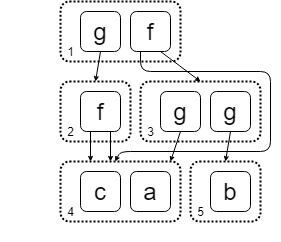
\includegraphics[width=\linewidth]{figures/egraph.png}
      \caption{}
      \label{fig:egraph}
    \end{subfigure}
    \begin{tabular}[b]{c}
      \begin{subfigure}[t]{0.45\columnwidth}
      \centering
        \begin{tabular}{|ccc|}
            \hline
            eclass-id & $\text{child}_1$ & $\text{child}_2$ \\
            \hline
            1         & 4        & 3        \\
            2         & 4        & 4       \\
            \hline
        \end{tabular}
        \caption{}
        \label{fig:repr-f}
      \end{subfigure}\\
      \begin{subfigure}[b]{0.5\columnwidth}
      \centering  
        \begin{tabular}{|cc|}
            \hline
            eclass-id & $\text{child}_1$ \\
            \hline
            1         & 2         \\
            3         & 4         \\
            3         & 5         \\
            \hline
        \end{tabular}
        \caption{}
        \label{fig:repr-g}
      \end{subfigure}
    \end{tabular}
  \end{tabular}
  \caption{(a) an e-graph over $T(\Sigma, \emptyset)$ and  $\cong_\Sigma$ where $\Sigma=\{f,g,a,b,c\}$ and $a,b,c$ are nullary functions. Each solid box denotes an e-node and each dashed box denotes an e-class. Every term represented by an e-class is mutually equivalent. For example, $a\cong_\Sigma c$, $g(a)\cong_\Sigma g(b)$, and $f(a, g(a)) \cong_\Sigma g(f(a, a))$. The labels of e-classes are at bottom left.\quad (b) relation representing $f$. \quad(c) relation representing $g$.}
\end{figure}

\paragraph{\Ematching.}
\Ematching is the task of finding \ematching substitutions that instantiate patterns to set of terms represented in the \egraph. 
An \textit{\ematching substitution} $\sigma$ is a function that maps every variable in a pattern to e-classes.
For convenience, we use $\sigma(p)$ to denote the set of terms obtained by replacing every occurrence of variable $v_i$ in $p$ with terms in $\sigma(v_i)$.
Formally, given an e-graph $E$ and a pattern $p$,  \ematching finds the set of all possible pairs $(\sigma, r)$ such that every term in $\sigma(p)$ is represented in the e-class $r$.
Terms in $\sigma(p)$ are said to be matched by pattern~$p$. $r$ is said to be the root of matched terms.
For instance, pattern $f(\alpha, g(\alpha))$
 matches four terms in e-class $c_1$: $f(a, g(a))$, $f(a, g(c))$, $f(c,g(c))$, and $f(c, g(a))$; 
 all of which are witnessed by the substitution $\{\alpha \mapsto c_4\}$.

Existing approaches to e-matching rely on backtracking \citep{efficient-ematching,simplify,egg}. 
For example, \citet{efficient-ematching} proposed a backtracking-based e-matching algorithm that is used by \textsc{Z3} \citep{Z3} and \egg \citep{egg}, two state-of-the-art e-graph implementations. 
To match the pattern $f(\alpha, g(\alpha))$ on the e-graph in Figure \ref{fig:egraph}, their algorithm does a depth-first search over the e-graph:
% Conceptually, it recursively searches for the pattern $f(\alpha, g(\beta))$ and filters out substitutions that map $\alpha$ and $\beta$ to different e-classes.
it searches for all $f$-application e-nodes $n_f$, adds $\alpha\mapsto n_f.\textit{child}_1$ to substitution $\sigma$, iterates through all $g$-application e-nodes $n_g$ in e-class $n_f.\textit{child}_2$, and only yield $\sigma$ if $n_g.\textit{child}_1=\sigma(\alpha)$.
In general, this procedure runs in time that is quadratic of the \egraph size.
In a large e-graph, there may be thousands of pairs of $n_f$ and $n_g$ where $n_g$ is in e-class $n_f.\textit{child}_2$, but only a few satisfy the constraint $n_f.\textit{child}_1=n_g.\textit{child}_1$. Therefore, backtracking-based \ematching enumerates an unnecessarily large pool of candidates.
Even worse, complex query patterns may involve many variables that occur at several places, which makes na\"ive backtracking enumerates an excessive number of terms and therefore extremely slow. 
This inefficiency is due to the fact that na\"ive backtracking does not use the equality constraints to prune the search space \textit{globally}. 
This is in contrast to our approach, which exploits the equality constraints during query planning for greater performance and guarantees worst-case optimality with respect to the output size.
  

\section{Conjunctive queries}

\paragraph{Relational schema.}
A relational schema $S_D$ over domain $D$ is a set of relation symbols with associated arities. An atom under a schema $S_D$ is an expression $R(t_1,\ldots,t_k)$, where $k$ is the arity of $R$ in $S_D$ and $t_i$ is an element in $D$. An instance of $S_D$ is a set of atoms over $S_D$. 

\paragraph{Conjunctive queries.}
A conjunctive query over schema $S_D$ and a set of variables $V$ is a formula of the form
\[
    \textit{ans}(x_1,\ldots x_k)\textit{ :- } R_1(v_{1,1},\ldots,v_{1,k_1}),\ldots, R_n(v_{n,1},\ldots,v_{n,k_n}),
\]
where $n\geq 0$, $R_1\ldots R_n$ are relation names in $S_D$ with arities $k_1,\ldots k_n$, \textit{ans} is the name of the resulting relation not in $S_D$, $v_{i,j}$ are variables in $V$\footnote{Some definitions of conjunctive queries allow both variables and constants, but we only allow variables in conjunctive queries for simplicity.}, and $x_1,\ldots x_k$ are variables occurring in $v_{i,j}$. We call such $R_i(v_{i,1},\ldots,v_{i,k_1})$ an atom of the conjunctive query.

\paragraph{Semantics of conjunctive queries.} 
Similar to \ematching substitutions, we define a conjunctive query substitution as a function that maps every variable occurring in $v_{i,j}$ to elements in $D$. The semantics of conjunctive queries is defined as follows: Let $q$ be a conjunctive query, $I$ be an instance of $S_D$, conjunctive queries yield the set of all $\textit{ans}(\sigma(x_1),\ldots,\sigma(x_k))$ where $\sigma$ is a substitution satisfying that $R_i(\sigma(t_1),\ldots \sigma(t_k))$ are atoms in $I$ for $i=1,\ldots,n$. We denote the result set as $q(I)$.

We make the observation that the definition of conjunctive query and \ematching
are definitionally similar to each other: both are defined as finding
substitutions whose instantiations are present in a (relational or graph)
database. In fact, the \ematching problem can be viewed as a ``nested''
conjunctive queries on a database where the atoms are nested. Therefore, it is
tempting to reduce the \ematching problem to a conjunctive query over the
relational database, thereby benefiting from well-studied techniques from the
database community, including join algorithms, query optimization, and query
evaluations.

\section[The AGM bound]{The AGM bound and Generic Join \footnote{This section is inspired by Remy Wang's \href{https://gitlab.com/remywang/blog/-/blob/master/posts/wcoj.md}{introduction to generic join algorithms}.}}

\algrenewcomment[1]{\(\triangleright\) #1}
\algnewcommand{\LineComment}[1]{\State \(\triangleright\) {\it #1}}
\paragraph{The AGM Bound}
\begin{figure}
  \centering
\begin{algorithmic}[1]
\Procedure{SolveTriangleQuery}{$R,S,T$}
\State $A := R(x,y).x \cap T(z,x).x$\;
  \LineComment{Compute $Q(\alpha,y,z) \textit{ :- } R(\alpha,y),S(y,z),T(z,\alpha)$}
  \For{$\alpha\in A$} 
  \State $B := R(\alpha,y).y \cap S(y,z).y$\;
    \LineComment{Compute $Q(\alpha,\beta,z) \textit{ :- } R(\alpha,\beta),S(\beta,z),T(z,\alpha)$}
    \For{$\beta \in B$}
        \State $C := S(\beta,z).z \cap T(z,\alpha).z$\;
        \LineComment{Yield join results $Q(\alpha, \beta, \gamma)$}
        \For{$\gamma \in C$}
        \State {\bf output } $Q(\alpha,\beta,\gamma)$
        \EndFor
    \EndFor
  \EndFor
\EndProcedure
  \caption{Generic join algorithm for the triangle query $Q(x,y,z) \textit{ :- } R(x,y),S(y,z),T(z,x)$, with ordering $[x, y, z]$.}\label{alg:gj}
\end{algorithmic}
\end{figure}

Given a database and a conjunctive query, the AGM bound \cite{agm} is a bound on how large the query output could be. A simple bound just multiplies the cardinally of each relation, which is the size of the Cartesian product of all relations. 
For example, for triangle query $ Q(x,y,z) \textit{ :- } R(x,y), S(y,z), T(x,z)$, this  bound computes to $|Q| \leq |R| \times |S| \times |T|$. 
If $|R|=|S|=|T|=N$, then $|Q| \leq N^3$.
However, we can do better: we observe that $Q$ contains fewer atoms than the query
$ Q’(x,y,z)\textit{ :- } R(x,y), S(y,z),$ as $Q$ is further filtered by joining with $T$. Therefore, we know $|Q| \leq |R| \times |S| = N^2$. 
In fact, the theoretical bound of conjunctive query output size is given as the AGM bound \citep{agm}, which is $N^{3/2}$ in this case.

The AGM bound proposes a question: is there an algorithm that always achieves the performance described by the AGM bound? In particular, \textit{cyclic queries} is a kind of conjunctive queries whose query hypergraph contains cycles, such as the triangle query $Q$ above, and they are known to make traditional join plans (e.g., join plans using two-way joins like hash joins or merge joins) suboptimal. Most of real-world database systems therefore have bad performance on cyclic queries.

\paragraph{Generic join.} Fortunately, theoretical progress has been made in the database theory community to achieve optimal performance on conjunctive queries and on cyclic queries in particualr. In particular, the generic join algorithm for conjunctive query is developed that runs in time linear to the worst-case output size with a log factor \citep{wcoj}. 
The generic join algorithm has great performance in practice when the query is cyclic, and is competitive to traditional join algorithms in other cases.
Given a conjunctive query and a relational database, generic join is parameterized over a ordering of the set of variables in the query, say $[x,y,z]$ for the query above. The ordering does not matter for the optimality guarantee, but may impact practical performance greatly. 
Given an ordering,
we assume the input relations are stored in tries sorted by the ordering.
That is, given the ordering $[x,y,z]$,
$R(x,y)$ is sorted by $x$ and then $y$,
and the first-level trie nodes are the $x$'s.
% Even more concretely,
% Figrue~\ref{fig:trie} illustrates the trie
% representing $R=\{(3, 4), (2, 1), (2, 5)\}$.
We can very efficiently intersect (join) relations on their
first (according to the variable ordering) variable given such tries.
Algorithm~\ref{alg:gj} shows the generic join algorithm for computing $Q$.
Note that selection, e.g. $R(a, y)$ is very fast with the built tries.
$A \cap B$ can also be done in $\tilde{O}(\min(|A|, |B|))$ time
($\tilde{O}$ means $O$ with a log factor).
For general queries we may have to intersect more than two relations,
in which case the intersection should be performed in
$\tilde{O}(\min_i|A_i|)$ time (using the merge in merge-sort).

\chapter{Relational E-matching}


\begin{figure}
    \centering
    % \caption{The main algorithm}\label{alg:main}
    \begin{algorithmic}[1]
    \Procedure{RelationalEMatching}{$E,\textit{ps}$}
    \State $\textit{I}\gets \textsc{EgraphToDatabase}(E)$
    \State \Return $\{\textsc{EvalCQ}(q, I)\ |\textbf{ for } p\in \textit{ps}, q\gets \textsc{PatternToCQs}(p)\}$
    \EndProcedure
    \end{algorithmic}
    \caption{The relational \ematching algorithm}
    \label{fig:main}
\end{figure}

\begin{figure}
    \centering
    \begin{align*}
        \textsc{EgraphToDatabase}(E) &= \{\textsc{EnodeToAtom}(n)\ |\text{ for \enode\ } n\in E\}\\
        \textsc{EnodeToAtom}(f(c_1,\ldots,c_n)) &= R_f(\textit{lookup}(f(c_1,\ldots,c_n)), c_1,\ldots, c_n)
    \end{align*}
    \caption{Transforming \egraphs to relational database}
    \label{fig:egraph_to_db}
\end{figure}

\def\aux{\textsc{Aux}}
\def\compile{\textsc{Compile}}
\begin{figure}
\begin{align*}
  \compile(p) &= Q(\textit{root}, v_1,\ldots,v_n) \leftarrow A\\
  &\quad \begin{aligned}
  \text{ {where} $v_1\dots v_n$ are variables in $p$}\\
  \text{{ and} $\aux(p)=\textit{root}\sim A$}\\
  \end{aligned}\\
  \aux(f(p_1,\ldots, p_n)) &= v \sim R_f(v, v_1, \ldots, v_n), A_1, \ldots, A_n \\
  & \text{\quad { where} $v$ is fresh and }\aux(p_i) = v_i \sim A_i \\
  \aux(x) &= x \sim \emptyset \text{\qquad { where} $x$ is a pattern variable}\\
\end{align*}
\caption{Compiling a pattern to a conjunctive query.}\label{alg:compile}
\end{figure}
In this chapter, we introduce our relational \ematching algorithm, shown in \autoref{fig:main}. 
The algorithm takes an e-graph $E$ and a set of patterns $\textit{ps}$. 
It first transforms the \egraph to its relational representation, denoted as $I$. 
Next, for each pattern, it compiles the pattern to a conjunctive query $q$, and executes this conjunctive query over $I$. 
This is particularly suited for scenarios like equality saturation. 
In such scenarios, the program optimizer switches between e-matching and batched rewrite applications in each iteration to amortize the run-time required for maintaining the congruence invariant, a technique known as ``rebuilding'' \citep{egg}. 
In such scenarios, the run time for materializing the \egraph can be neglected compared to the \ematching workload.
In other scenarios, where the \egraph is frequently updated and \ematching is performed interactively, it is possible to use a totally relational representation to avoid the cost of frequent materialization of the relational database and use standard update operations from a SQL-like language\footnote{We actually implemented a prototype \egraph purely on top of an in-memory relational database that does not use graph data structure nor union-finds.}.
However, we suspect this would incur a larger constant factor to the run time compared to the graph representation of \egraph.
In general, we left the problem of interactive \ematching, where \ematching is performed on a frequently updated \egraph, as future work (See Chapter~\ref{sec:future}).

\section{Reducing e-graphs to relations}

The first step of relational e-matching is to transform the \egraph to a relational database. 
An \egraph $E$ representing a congruence relation over $T(\Sigma,\emptyset)$ will be mapped to a relational database over \id, the set of \eclass ids. 
For every $n$-ary symbol $f$ in $\Sigma$, We map it to an $n+1$-ary symbol $R_f$ in schema $S_\id$.
We refer to fields of $R_f$ as $\eclassid,\child_1,\ldots,\child_n$ respectively, and they denote the \eclass this \enode belongs to and the children \eclasses of this \enode respectively.
For every \enode in the \egraph, we map it to an atom in the relational database.
The algorithm is presented in \autoref{fig:egraph_to_db}. 

Take the \egraph in \autoref{fig:egraph} for example. There are 8 \eclasses in total. The $g$-application \enode in \eclass $c_1$ translates to atom $R_g(1, 2)$, where $1$ is the id of the \eclass that contains it and $2$ is the id of its child \eclass. Similarly, the $f$-application \enode in \eclass $c_2$ translates to the atom $R_f(2, 4, 4)$, where $2$ is the id of the \eclass that contains it and $4,4$ are the ids of its child \eclasses. \autoref{fig:egraph_to_db} only shows the relation representing $f$ and $g$. The relations representing constants $a,b,c$, which are all relations with $\leq 1$ atom, are omitted for brevity.

\section{Reducing \ematching patterns to conjunctive queries}
\label{sec:pattern_to_cq}

We reduce every \ematching to a conjunctive query so that it can be run on the relational representation of \egraphs. 
We use the algorithm in \autoref{alg:compile} to ``unnest'' a pattern to a conjunctive query. The \aux{} function returns a variable and a conjunctive query atom list. 
Particularly, for non-variable pattern $f(p_1,\ldots p_n)$, \aux{} produces a fresh variable $v$ and a concatenation of $R_f(v, v_1,\ldots, v_n)$ and atoms from $A_i$, where $v_i\sim A_i$ is the result of calling $\aux(p_i)$. For variable pattern $x$, \aux{} simply returns $x$ and an empty list.
Given a pattern $p$, the \compile{} function returns a conjunctive query with body atoms from $\aux(p)$ and the head atom consisting of the root variable and variables in $p$. The compiled conjunctive query and the original \ematching query are equivalent because there is an one-to-one correspondence between the output of them. Specifically, each output atom of the form $Q(c_\textit{root}, c_{x_1},\ldots c_{x_k})$ denotes an \ematching output $\left(c_\textit{root}, \{x_1\mapsto c_{x_1},\ldots,x_k\mapsto c_{x_k} \}\right)$.

With this algorithm, the example pattern $f(\alpha, g(\alpha))$
 is compiled to the following conjunctive query $$Q(\textit{root},\alpha)\,\textit{:-}\,R_f(\textit{root},\alpha,x),R_g(x,\alpha).$$
Compared to the original \ematching pattern, this flattened representation enables the pattern search to utilize both the structural and the equality constraints. For example, most of the database optimizers will synthesize query plans that build and lookup indices on both join variables (i.e., $x$ and $\alpha$), which runs in linear time. In contrast,  backtracking-based \ematching takes quadratic time. Backtracking-based \ematching can be seen as a hash join that only builds and look-ups a single variable (i.e., $x$), and filter the outputs using the equality predicates on $\alpha$. In other words, existing \ematching algorithms will consider all $f(\alpha, g(\beta))$ regardless whether $\alpha$ is congruent to $\beta$, while the generated conjunctive query gives the query optimizer the freedom to synthesize query plans that will consider only atoms where $\alpha\cong\beta$.

\section{Answering conjunctive queries with generic join}


Finally, we consider the problem of efficiently solving the compiled conjunctive
queries. We propose to use the generic join algorithm to solve the generated
conjunctive queries. Although traditional query plans, which are based on two
way joins such as hash joins and merge-sort joins, are
extensively used in industrial relational database engine, they may suffer from
certain conjunctive queries \ematching~generates. For example, consider the
pattern $f(g(\alpha),g(\alpha))$. The synthesized conjunctive query
is $$Q(\alpha)\gets R_f(\textit{root}, x, y), R_g(x, \alpha), R_g(y, \alpha),$$
which is a cyclic conjunctive query. Two-way join plans suffer on these cyclic
queries because they are unable to leverage all the constraints in the
conjunctive query to prune the space during enumeration. Consequently, two-way
join plans will enumerate terms that do not satisfy the constraint and prune
them away \textit{a posteriori}. In contrast, the generic join algorithm will
only consider a concrete term when the term satisfies all the constraints.
Moreover, generic joins has comparable
performance on acyclic queries with two-way join plans. These properties make
generic join our ideal solver for conjunctive queries generated from \ematching
patterns.
\chapter{Discussion}

\section{Complexity and optimality}
\label{sec:disc:complexity}

Generic join guarantees worst-case optimality with respect to the output size.
Our relational \ematching preserves this optimality. In particular, we have the following theorem:
\newtheorem{theorem}{Theorem}
\begin{theorem}
Relational \ematching is worst-case optimal; that is, fix a pattern $p$, let $M(p,E)$ be the set of substitutions yielded by \ematching on an \egraph $E$ with $n$ nodes, relational \ematching runs in time $\tilde O(\max_E(|M(p,E)|))$.
\end{theorem}
\begin{proof}

Notice that there is an one-to-one correspondence between an output atoms of the generated conjunctive query and the \ematching. Therefore, the worst-case bound is the same across an \ematching pattern and the conjunctive query it generated. Because generic join is worst-case optimal, relational \ematching also runs in worst-case optimal time with respect to the output size.
\end{proof}


\section{Other join algorithms}

Although we choose generic join algorithm in relational \ematching, there are also other choices in the design space. For example, traditional two-way join plans are efficient on acyclic queries, and extensive research has been done on synthesizing highly efficient query plans. Moreover, Yannakakis' algorithm \citep{yannakakis} is an optimal algorithm on ayclic queries, running in time equal to the size of the output (with possible log factors). However, both of the queries suffer on cyclic conjunctive queries. Two-way join plans spend time enumerating unsatisfying terms, while Yannakakis' algorithm are not applicable to cyclic conjunctive queries. It is possible to choose different join algorithms based on the cyclicity of the query to take advantages each algorithms. However, we currently does not implement this.

\section{Comparison to graph pattern matching}

The idea of representing graph data structure as relational databases are not new. For example, many Datalog programs represent nodes and edges as their own relations to use relational joins to support efficient queries on graph database, known as graph pattern matching. Compared to the common encoding of graphs, our relational representation of \egraphs in a relational database is slightly different and specialized for \egraphs. It is a future work to absorb researches on graph pattern matching for relational \ematching.


\chapter{Implementation}

We implemented our relational \ematching algorithms for the \egg equality saturation framework. In this section, we describe several implementation details. 

\section{Overview}
Given an \ematching pattern, we first transform it to a conjunctive query using the algorithm described in Section \ref{sec:pattern_to_cq}. Next, we lower the conjunctive query to an execution plan, represented as a sequence of variables that the generic join will go through. The execution plan is reconstructed for every new \egraph, because the query compiler may depend on the statistics of the \egraph to generate the execution plan. We then build the indices for each atom $R(v_1,\ldots,v_k)$ in the Cconjunctive queryaccording to the variable ordering. Finally, we use an efficient interpreter to run the generic join algorithm.

\section{Variable Ordering}

Different variable ordering may result in asymptotically different performance \citep{eval-wcoj, emptyheaded}. 
Therefore, choosing an variable ordering is important. 
Compared to join plans for binary joins, there is few literature on query plans for generic joins.
Therefore, we developed two heuristics based on empirical experiment. 
First, we prioritize variables that are associated to more relations, because the intersected set of more relations are more likely to have a smaller cardinality. 
Moreover, we prioritize variables that are attached to small relations. 
By intersecting on these variables first, generic join could use the smaller relations to early prune a large portion of atoms in other relations that is not satisfying. 

Using these two constraints, the optimizer is able to find superior query plans than the top-down search of backtracking-based \ematching even for linear patterns, where our relational \ematching does not have more information than \ematching. 
For example, for queries like $x+\alpha$, our optimizer is able to exploit the fact that there is only one atom in the $R_x$ (i.e., the relation representing constant $x$), so enumerating this relation and use attributes of $R_x$ to prune $R_+$ will immediately produces all valid substitutions. Meanwhile, in the top-down fashion of backtracking-based \ematching, the matching procedure will need to go through all atoms of $R_+$ and check if constant $x$ resides in their second child. Such query plan examines much more unnecessary atoms in $R_+$, because only a small number of $+$-application \enodes are connected to $x$.

\section{Indexing}

The generic join assumes that indices are built for the given variable ordering. However, they are crucial to the actual performance of generic join \citep{eval-wcoj}.
We currently use a recursive trie structure for indexing. The trie is a hash map from the \eclass ids to itself. An atom is represented as a path from the root in the trie, according to the order of visiting. The indices are built on demand and shared among different \ematching pattern search on the same \egraph. For most non-trivial \ematching queries, the index building time is neglectable.
We believe there are still space for improvement surrounding indices, such as optimizing the set intersection operations and using a more cache-friendly representation.

\section{Other optimizations}

Finally, we write specialized implementations for various numbers of relations being intersected at each nested layer of generic join. This makes possible unrolling most of the loops when manipulating multiple relations together. Moreover, during index building, if the residual relation is known not to join with any other relations, we switch from trie to a flattened vector that directly stores the relation, which is more cache friendly and avoid backtracking during enumeration of the residual relation. In our experiment on handwritten queries, this optimization enables up to $4\times$ performance gain even on simple queries.
\chapter{Evaluation}

In this section, we first categorize \ematching patterns into three categories. Next, we evaluate our prototype of relational \ematching with two preliminary experiments, choosing patterns from each of the categories, and discussed our progress on evaluating full-system benchmarks. More experiment will be presented in the forthcoming paper.


To investigate the kinds of conjunctive queries an \ematching pattern would generate and its performance implication on the join algorithms, we categorize the \ematching patterns into three categories according to the kinds of conjunctive queries they generate:
\begin{enumerate}
    \item Linear patterns: this is the simplest form of patterns, where no variables occur more than once in the pattern. Examples of this category include $f(\alpha, \beta)$ and $f(g(\alpha),g(\beta))$).
    \item Non-linear acyclic patterns: we define non-linear acyclic patterns to be patterns that are not linear and satisfy that every multi-occurrence of a variable must occur between \enodes that has ``distance'' $\leq 1$ with each other. Examples of this category include  $f(\alpha,g(\alpha))$ and $f(f(\alpha,\beta), \alpha)$.
    \item Cyclic patterns: we define all other patterns to be cyclic patterns. Examples include $f(g(\alpha), g(\alpha))$ and $f(f(\alpha,\beta), g(\beta))$). Note that \ematching patterns of this category are always reduced to cyclic queries.
\end{enumerate}

All three categories of patterns exist in real-world applications like equality saturation. 
For example, the search patterns for commutative law (e.g., $a+b$) and associative law (e.g., $(a+b)+c$) is linear, and the search patterns for the distributive law (e.g., $a\times b+a\times c$) is cyclic, while that for the rule for reciprocal (e.g., $x\times (1/x)$) is non-linear acyclic.


We choose two benchmarks from the \egg's test suites, namely the math test suite, which saturates mathematical expressions, and the lambda test suite, which saturates lambda calculus terms. Both of them are representative of a standard application of equality saturation. For example, the math test suite has many overlapping rules with Herbie \citep{herbie}, an application of equality saturation in the domain of floating-point arithmetic.

We did two preliminary experiments. The first experiment tries to understand the asymptotic speedup of relational \ematching. In this experiment, we manually write the implementation for relational \ematching for three patterns, which are representative of linear patterns, non-linear acyclic patterns, and cyclic patterns. We benchmark against the \ematching algorithm in \egg, which implements the backtracking-based \ematching algorithm described in \citet{efficient-ematching}\footnote{In fact, \egg does not implement all of the instructions of the backtracking virtual machine described in \citet{efficient-ematching}, since some of the instructions and their compilation are very complicated.}, on different \egraph sizes.

\begin{figure}
    \centering
    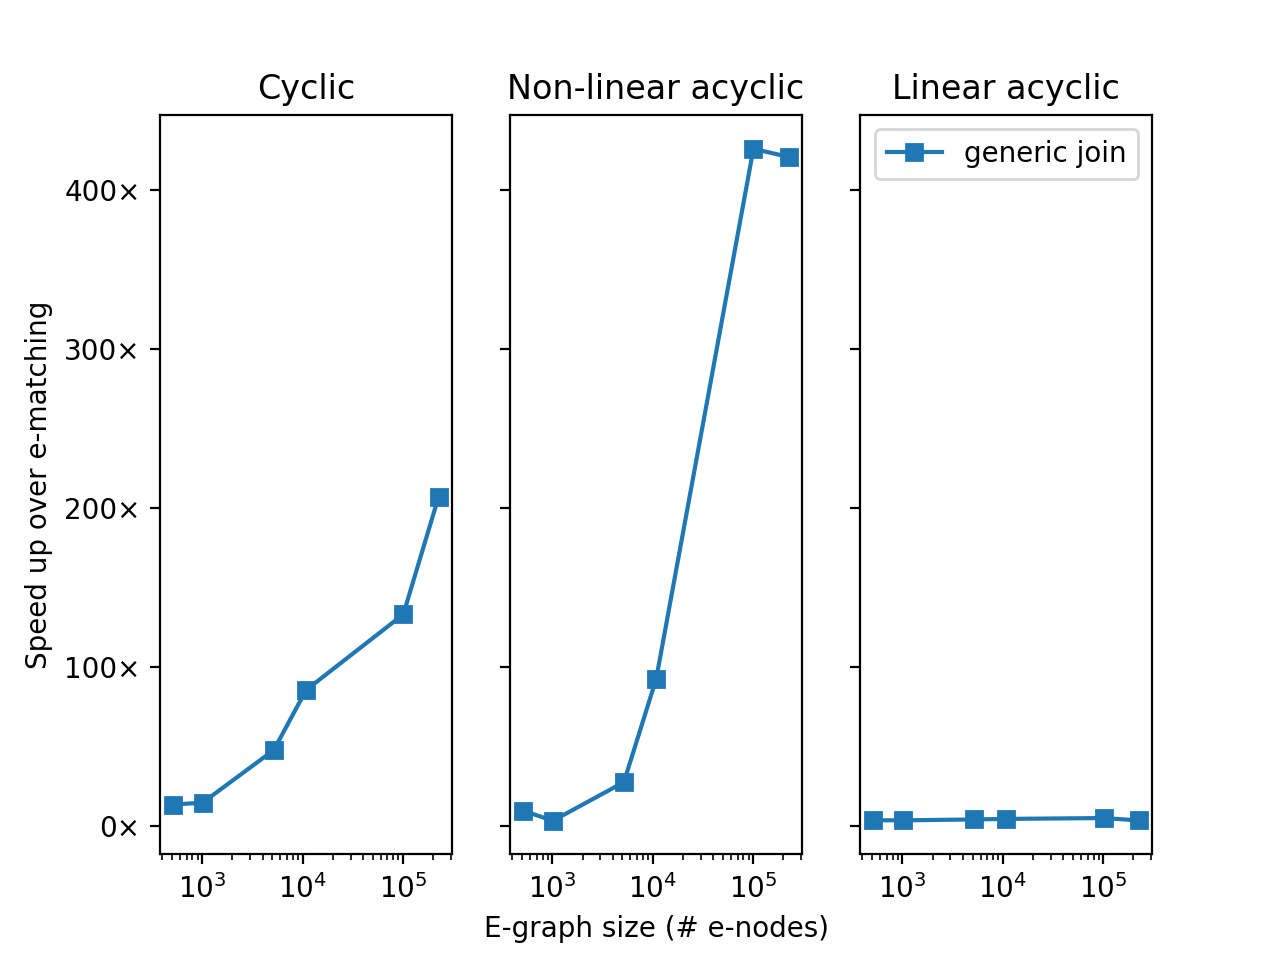
\includegraphics[width=\linewidth]{figures/egdb.png}
    \caption{Speedup of relational \ematching over backtracking-based \ematching algorithms}
    \label{fig:bench1}
\end{figure}

The result is shown in Figure \ref{fig:bench1}. On both cyclic and non-linear acyclic case, our relational \ematching achieves asymptotically better performance, up to 426$\times$, over backtracking-based \ematching by taking advantages of the equality constraints. In the linear
case, because no variable occurs more than once, relational \ematching
achieves similar performance as the backtracking-based \ematching up to a constant factor.\footnote{Note that the comparison here is between the handwritten relational \ematching, which is compiled, and the \ematching engine in \egg, which is interpreted, because this experiment is performed for the PLDI SRC, when we have not developed a fully working version of relational \ematching inside \egg. Therefore, the comparison is not perfectly apple-to-apple. However, we can still see the asymptotic trends.}

\begin{figure}
\vspace{-4em}
     \centering
     \begin{subfigure}[b]{0.8\textwidth}
         \centering
         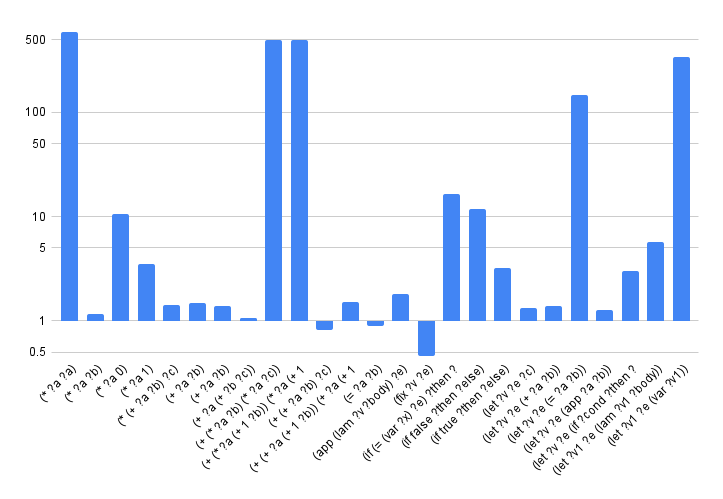
\includegraphics[width=\textwidth]{figures/bench2-1.png}
         \caption{}
         \label{bench2-1}
     \end{subfigure}
     \\
     \begin{subfigure}[b]{0.8\textwidth}
         \centering
         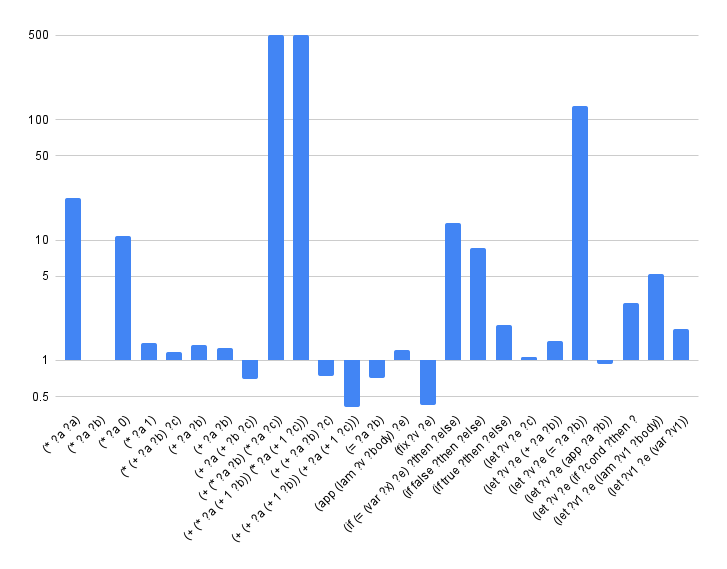
\includegraphics[width=\textwidth]{figures/bench2-0.png}
         \caption{}
         \label{bench2-0}
     \end{subfigure}
     \caption{(a) Speedup of relationl \ematching over backtracking-based \ematching on microbenchmarks without index building time. (b) Speedup of relationl \ematching over backtracking-based \ematching on microbenchmarks with index building time.}
     \label{bench2}
\end{figure}


Next, we compare the performance of relational \ematching as we implemented in \egg against \egg's original \ematching implementation on several benchmarks. The result is presented with two figures in Figure \ref{bench2}. Figure~\ref{bench2-1} only compares the enumeration procedure of backtracking-based \ematching to that of relational \ematching, excluding time that may need to build the index before performing generic join, which are shared among different patterns, and Figure~\ref{bench2-1} makes the same comparison but includes the index building time.

According to Figure~\ref{bench2-1}, relational \ematching achieves substantial speedups for complex patterns. However, on some simple patterns, relational \ematching does not achieve a significant speedup compared to backtracking-based \ematching algorithms, and sometimes relational \ematching is slower.
Most of such patterns are linear patterns like \texttt{(+ (+ ?a ?b) ?c)} and \texttt{(fix ?v ?e)}. In particular, patterns like \texttt{(fix ?v ?e)} are equivalent to a simple enumeration of all $f$-application terms for some function symbol $f$, which we call singleton patterns. The relational \ematching has the most slowdown on several singleton patterns because running singleton patterns is very fast, taking only a few microseconds, so the overhead related to relational \ematching such as query compilation dominates the run time. Still, because they only take a few microseconds, the run time for matching such patterns are not an issue for real applications. Moreover,  note the relational \ematching performs order of magnitude  better on pattern \texttt{(* ?a ?a)}, which is a singleton pattern, as our query optimizer exploits the fact that both children of the *-application node are the same and thus only does a filter over the corresponding relation. In contrast, backtracking-based \ematching without ad hoc handling can only express this as a backtracking process, which has a larger overhead.

Comparing Figure~\ref{bench2-1} against  Figure~\ref{bench2-0}, we observe the time taken for building indices to be significant. Many plans where relational \ematching is faster now becomes slower. This is consistent with the observation made by \cite{eval-wcoj}, where index building is sometimes the bottleneck of the generic join algorithm. Since our current implementation is only a prototype, we are currently working on improving the index building time so that the performance of relational \ematching is able to dominate that of the current implemented \ematching in \egg.
 
Finally, our next step of experiment is to evaluate relational \ematching on full-system applications that use \egg. We attempted to run Herbie with relational \ematching as the \ematching procedure. However, we are unable to observe any significant speedup by using relational \ematching. We speculate the cause is that the workload of Herbie is running only simple, linear patterns on small \egraphs, so there are no additional equality constraints that relational \ematching could exploit. We are working on evaluating relational \ematching on other applications, such as Tensat \citep{tensat} and Szalinski \citep{2020-pldi-szalinski-cad-eqsat}.
\chapter{Conclusion}

Existing \ematching algorithms are based on backtracking and suffer from problems like implementation difficulty, run inefficiency, and a loose complexity bound. To tackle these problems, we propose relational \ematching, an algorithm that efficiently solves the \ematching problem by reducing it to conjunctive queries. Relational \ematching is based on the observation that \ematching is definitionally similar to conjunctive queries. Leveraging this observation, relational \ematching maps an \egraph to a set of relations and compiles every \ematching pattern to a conjunctive query. As conjunctive query has been extensively studied in the database community for decades, relational \ematching is \textit{conceptually simpler}. Moreover, such relational representation provides an unified way to express not only structural constraints, but also equality constraints, which are constraints that backtracking-based \ematching fails to take advantage of during query planning. By exploiting equality constraints, relational \ematching performs \textit{asymptotically faster }than existing\ematching algorithms on many queries. Finally, to avoid enumerate an unnecessarily large space of candidates, relational \ematching uses generic join to solve the generated conjunctive queries, which makes relational \ematching \textit{worst-case optimal}.

We implemented relational \ematching in \egg and evaluate our relational \ematching on some microbenchmarks. Preliminary experiment indicates that relational \ematching shows asymptotic speedup over backtracking-based \ematching algorithms on both cyclic and nonlinear acyclic patterns. However, for linear patterns, relational \ematching shows similar performance as backtracking-based \ematching algorithms, up to a constant factor. In the future, we plan to evaluate relational \ematching more extensively and on more realistic \egraph applications.
\chapter{Future works}
\label{sec:future}
We believe there is a deep connections between \egraphs and relational dabase and \egraph can really benefit from research fruits of the database community. This thesis is only a very first attempt to bridging \egraphs and relational databases. Many things are left to be done. This sections sketches a few future works that are worth investigating. Some of them are technical, while others require insights into both areas.

\paragraph{Experiments.}
The current experiments are still very preliminary. To fully explore the design space of various join algorithms (e.g., hash join, Yannarakis' join algorithm) and query optimization strategies (e.g., different variable ordering for generic join, as well as standard optimization techniques for relational queries) for the scenarios of \ematching.

\paragraph{Multi-patterns.} A common extension to \ematching is multi-patterns \citep{efficient-ematching}. Multi-patterns generalize single patterns to multiple patterns that share the the same of variables. For example, $\alpha \times \beta, \alpha\times \gamma$ is a multi-pattern that searches for substitutions $\sigma$ that satisfy $\sigma(\alpha\times\beta)$ and $\sigma(\alpha\times\gamma)$ are both present simultaneously. They are extensively used in SMT solvers and are also useful in various equality saturation scenarios. Specialized algorithms are developed for multi-patterns. However, from a relational perspective, the conjunctive query generated by a multi-pattern is just a sequence of conjunctive query atoms generated from each pattern placed together. Therefore, the relational \ematching naturally generalizes to the scenarios of multi-patterns.

\paragraph{Optimizing query plans for generic joins.} There are not as many research done on optimizing the variable ordering as on optimizing traditional join plans. EmptyHeaded is the first graph database engine that uses generalized hypertree decompositions (GHD) to optimize generic join and achieves performance similar to low-level graph engines. However, it only focuses achieves a stronger run-time worst-case optimality guarantee, but does not take variable ordering into considerations. Yet it has been shown different variable ordering may leads to asymptotically different results \citep{eval-wcoj}. Therefore, it is one of our future directions to design algorithms to search for an optimal variable orderings during query optimization.

\paragraph{\Egraph engine purely on relational databases.} This paper only exploits the possibility of doing \ematching on a relational representation of \egraphs. It is our assumption that normal \egraph operations like merge and lookup are still done on the original \egraph representation and the relational representation will be re-computed during each (batch of) \ematching.   However, it is possible to build an \egraph engine purely on top of relational databases by canonicalizing every \enode on the fly during merge. Although we expect it incurs performance penalty to use a purely relational database to describe \egraph and operations on \egraph, it is ideal for situations where interactive \ematching is required. In such cases, it is unrealistic to rebuild the relational representation for every \ematching invocation, while such cost can be avoided if all \egraph operations are directly applied to its relational representation. Moreover, by describing every \ematching operations in terms of the language of relational databases, it is possible to benefit from the literature on incremental maintenance of relational databases and design an algorithm for {\it incremental} \ematching.

\paragraph{Exploring functional dependency for relational \ematching.} Functional dependencies are constraints such as two atoms having the same value on attributes $\textit{attr}_1,\ldots \textit{attr}_{n-1}$ implies they also share the same value on attribute $\textit{attr}_n$. Functional dependency are ubiquitous in relational databases, and they are also present in the relational representation of \egraphs. In particular, For a relation $R_f(\textit{eclass-id},\child_1,\ldots,\child_k)$ representing $f$, the value of $\textit{eclass-id}$ are determined by the values of $\child_1,\ldots \child_k$.

Our current relational \ematching does not take functional dependencies into considerations, but they may have an impact on the bound of worst-case output. Fortunately, there are worst-case optimal join algorithms that guarantee optimality with the presence of functional dependencies. Therefore, it is worth incorporating functional dependencies into relational \ematching and derives a tighter worst-case bound for relational \ematching.

\paragraph{Datalog engine with internalized congruence.} 
One of our initial motivation for this work is to develop a more flexible language for \egg. Tasks in \egg are described as rewrite rules that add the rewritten terms into the same \eclass as the matched terms. Therefore, \egg only supports equivalence reasoning, and it is very hard to describe relations that are not symmetric, such as a transitive closure. However, such directed relations are prevalent in real-world applications. One idea is to make the \egraph engine an extension of the Datalog language \citep{datalog-survey}. Datalog is a logic programming language that can be efficiently evaluated, and many relational properties such as transitivity, reflexivity, and symmetry can be naturally expressed in Datalog.
However, many relations, such as the equivalence relation, may be asymptotically slower if directly expressed in Datalog compared to a dedicated data structure.
Souffl\'e is a Datalog tool that support efficient equivalence relations as a specialized relation and uses an efficient union-find data structure to maintain equivalence relations.
Therefore, it is desired to extend Datalog language to efficient maintain congruence closures. On the one hand, this extends the equivalence reasoning in \egraphs to other kinds of reasoning as well. On the other hand, it makes certain existing Datalog programs efficient by using a more dedicated data structure.

 
% ========== Chapter 2
 
\printendnotes

%
% ==========   Bibliography
%
\medskip

\bibliographystyle{ACM-Reference-Format}
\bibliography{uwthesis}


\end{document}
